% vim:ft=tex:
%
\documentclass[12pt]{article}
\usepackage[utf8]{inputenc}
\usepackage[T1]{fontenc}
\usepackage[pdftex]{hyperref}
\usepackage{graphicx}
\usepackage{float}
\usepackage[dvipsnames]{xcolor}

\title{VulnBox: 1}
\author{Gz}
\date{}

% settings
%% hyperref
\hypersetup{
    colorlinks = true,
    linkcolor = blue,
    urlcolor = cyan
}
%% graphicx
\graphicspath{
    {./pics/}
}
%% indent
\setlength{\parskip}{0.5em}

\begin{document}
\maketitle
\tableofcontents
\pagebreak

%\section{Preparation}
\section{About the box}

    This is a \textbf{b2r} (\textit{boot2root}) easy/medium machine challenge
    which intends to show some common but less known features like \texttt{sg},
    \texttt{doas} and \texttt{cmp}.

    Requirements:
    \begin{itemize}
        \item Web enumeration
        \item Medium SQLi exploitation
        \item Linux knowledge
        \item System enumeration
        \item Hash cracking
    \end{itemize}

\section{Solution}

    The machine is an easy level, but not that straightforward, it's intended
    to work with tools or techniques I've seen very little out there so far.

\subsection{Reconnaissance and Enumeration}

    Let's get started by discovering the IP address of our target:

    \begin{figure}[H]\label{pic:01-host-discovery}
        \centering
        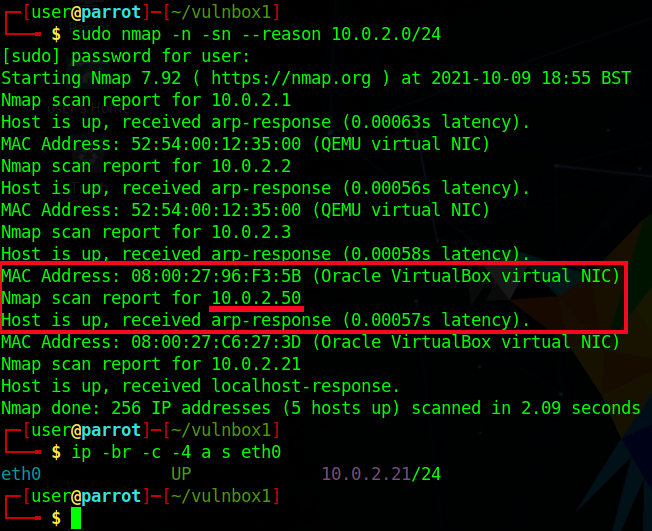
\includegraphics[width=1.00\textwidth]{01-host-discovery-gimp.png}
        \caption{Host Discovery with \texttt{nmap}}
    \end{figure}

    My IP address is \texttt{10.0.2.21}, the first three are from
    \textit{VirtualBox}, and the remain one is our target's
    (\texttt{10.0.2.50}).

    Let's see what ports it has open. I start with \textbf{TCP} ports as most
    services leverage this protocol because of its reliability. If we didn't
    find anything interesting we'd move on and would scan the \textbf{UDP}
    ports.

    \begin{figure}[H]\label{pic:02-nmap-tcpPorts}
        \centering
        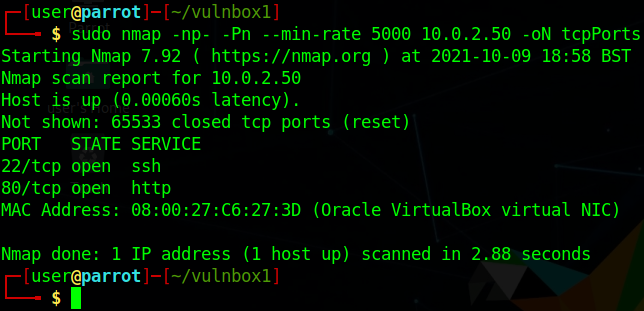
\includegraphics[width=1.00\textwidth]{02-nmap-tcpPorts.png}
        \caption{Port Scanning: \textbf{TCP}}
    \end{figure}

    We know now what ports are open, and they might be our possible way in.
    \texttt{nmap} shows those ports with the \textit{default} protocol
    associated. Which in most cases matches the reality, but in some others,
    they don't. They may be changed to be ``\textit{hidden}''\footnote{This is
    known as ``\textit{Security through obscurity}''.}.

    However, \texttt{nmap} can perform more advanced scans to fingerprint the
    services according to the responses received:

    \begin{figure}[H]\label{pic:03-nmap-tcpServices}
        \centering
        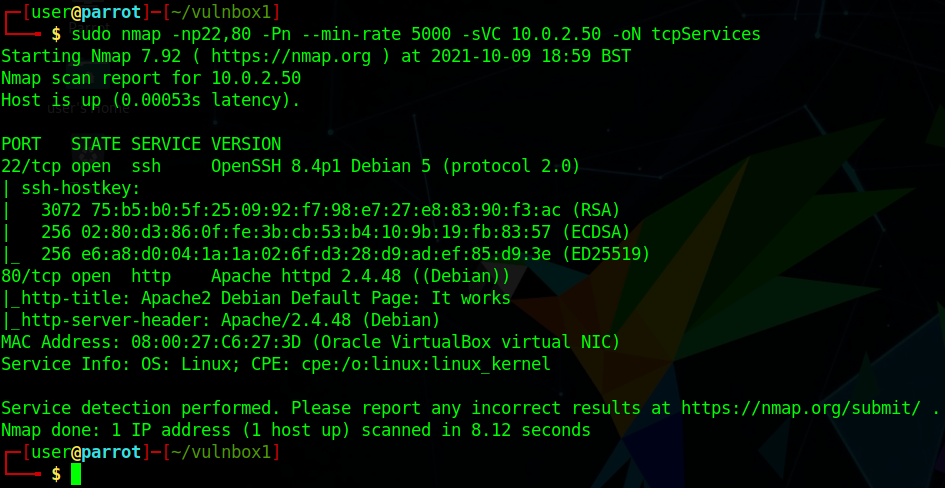
\includegraphics[width=1.00\textwidth]{03-nmap-tcpServices.png}
        \caption{Service Fingerprinting: \textbf{TCP}}
    \end{figure}

    We've got some important information already:
    \begin{itemize}
        \item \verb!22/tcp: OpenSSH 8.4p1 Debian 5 (protocol 2.0)!
        \item \verb!80/tcp: Apache httpd 2.4.480 (Debian)!
    \end{itemize}

    We're before, what it looks like, a \textit{Debian} distro. And we know the
    versions of both the \textbf{SSH} and web server.

    Since there's a web server, we can use a web browser to see the contents:

    \begin{figure}[H]\label{pic:04-browser}
        \centering
        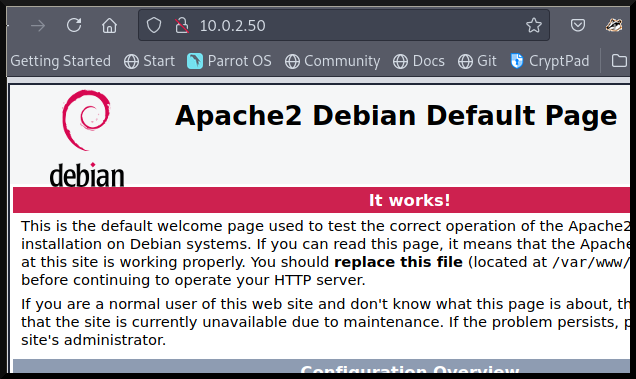
\includegraphics[width=1.00\textwidth]{04-browser.png}
        \caption{Initial page: \textit{Apache}'s default page}
    \end{figure}

    This is the \textit{Apache}'s default page. We can use \texttt{whatweb} to
    see quickly if there's a technology in use we don't see:

    \begin{figure}[H]\label{pic:05-whatweb}
        \centering
        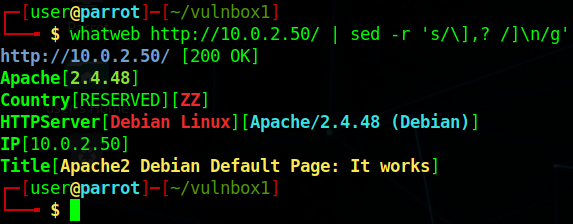
\includegraphics[width=1.00\textwidth]{05-whatweb-80.png}
        \caption{\texttt{whatweb} output on the initial page}
    \end{figure}

    Nothing out of the ordinary.

    We have no choice but start fuzzing. Let's start with possible resources. To
    save time I try to search with the extensions \texttt{.txt}, as it's a very
    common extension in any operating system I can think of, and \texttt{.php}, 
    as the web server is \textit{Apache}, and its web applications are commonly
    written in this language.

    \begin{figure}[H]\label{pic:06-ffuf}
        \centering
        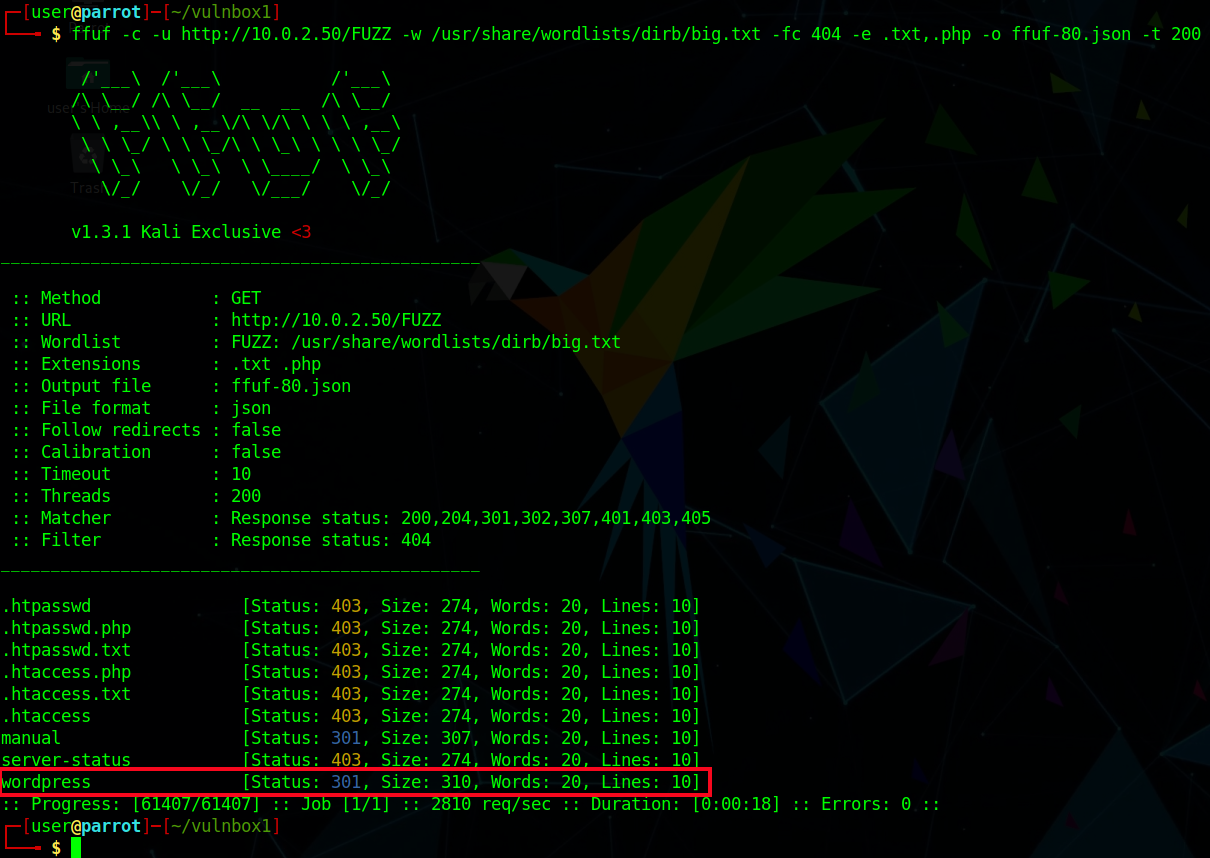
\includegraphics[width=1.00\textwidth]{06-ffuf-80-gimp.png}
        \caption{Fuzzing ``hidden'' resources with \texttt{ffuf}}
    \end{figure}

    The \textbf{wordpress} resource catches my eye immediately. We see its
    contents on a web browser:

    \begin{figure}[H]\label{pic:08-browser-wordpress}
        \centering
        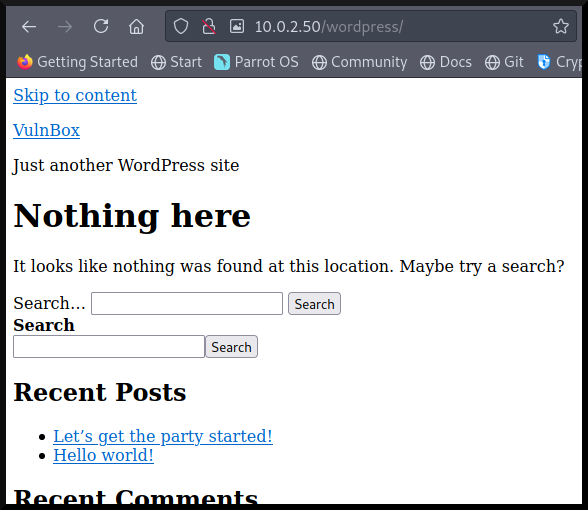
\includegraphics[width=1.00\textwidth]{08-browser-wordpress.png}
        \caption{\textit{WordPress} main page}
    \end{figure}

    It doesn't look right. It might be using \textit{virtual hosting}, we can
    see this either by hovering on the links or by inspecting the source page:

    \begin{figure}[H]\label{pic:09-browser-src-wordpress}
        \centering
        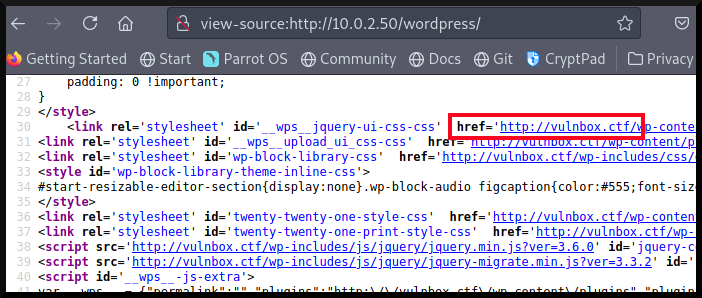
\includegraphics[width=1.00\textwidth]{09-browser-src-wordpress.png}
        \caption{\textit{WordPress} main page \textbf{HTML} source code}
    \end{figure}
    
    It seems it makes requests to \texttt{vulnbox.ctf}, let's check its
    behaviour with a plain requests and another specifying the domain found in
    the \texttt{Host} header:

    \begin{figure}[H]\label{pic:10-curl-host}
        \centering
        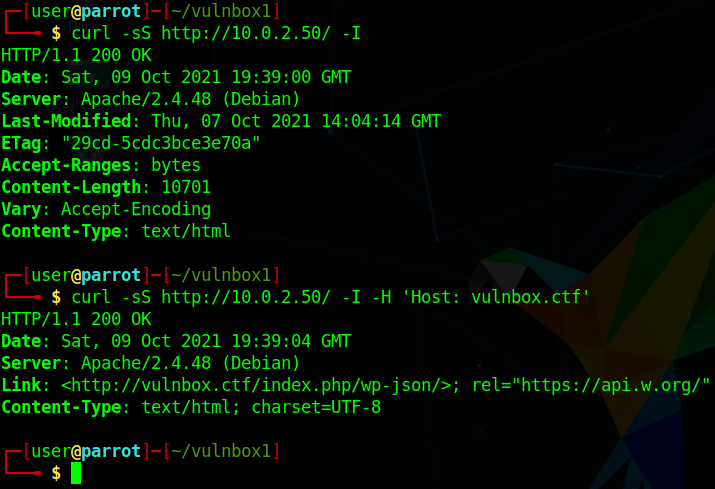
\includegraphics[width=1.00\textwidth]{10-curl-host.png}
        \caption{Difference between using the IP or the domain}
    \end{figure}

    The response is clearly different. This may mean \textit{virtual hosting}
    is being applied. We should add it to \texttt{/etc/hosts} so the domain is
    resolved to our target IP address.

    This way we can browse the web through our web browser seeing the contents
    intended to be shown.

    \begin{figure}[H]\label{pic:11-getent}
        \centering
        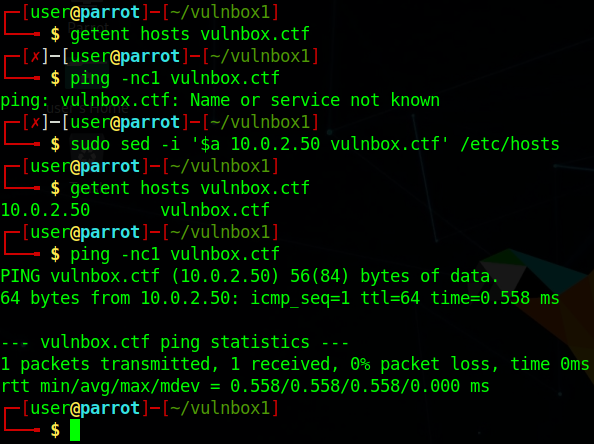
\includegraphics[width=1.00\textwidth]{11-getent.png}
        \caption{Adding the domain to \texttt{/etc/hosts}}
    \end{figure}

    Navigating to \texttt{vulnbox.ctf} on the web browser we see:

    \begin{figure}[H]\label{pic:12-browser-vulnbox}
        \centering
        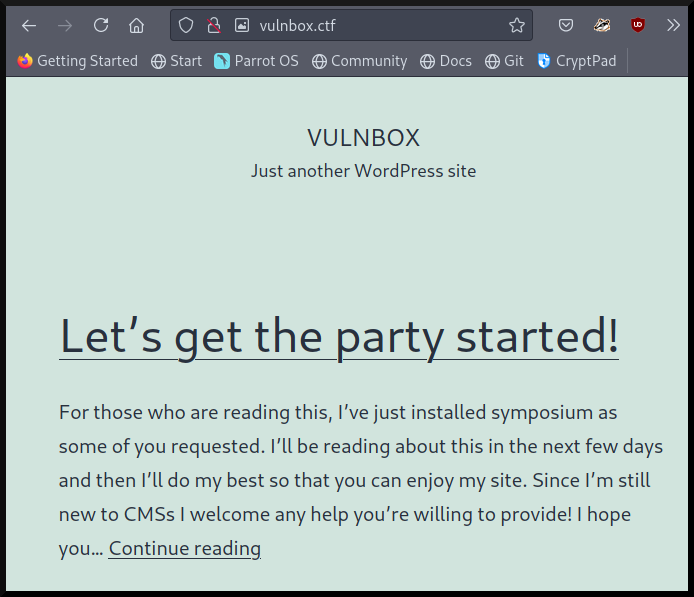
\includegraphics[width=1.00\textwidth]{12-browser-vulnbox.png}
        \caption{\textit{WordPress} blog}
    \end{figure}

    \textit{Et voilà !} we see the page correctly.

    Within this blog post, we can extract some crucial information. On the one
    hand, we have a username, namely, \textbf{albert}, who said he's installed
    something. That should make us think he's got some sort of privileges. On
    the other hand, he's saying what he's installed: \textbf{symposium}:

    \begin{figure}[H]\label{pic:13-browser-albert}
        \centering
        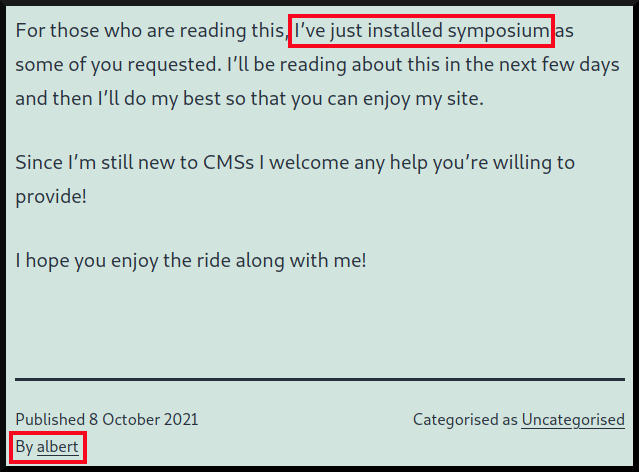
\includegraphics[width=1.00\textwidth]{13-browser-albert.png}
        \caption{Information Gathering from the blog post}
    \end{figure}

    To confirm if the username found is valid, we should try to log in, the
    usual path for \textit{WordPress} log in is in
    \verb!{WORDPRESS}/wp-login.php!, if we go there we'll see objective panel.

    \begin{figure}[H]\label{pic:14-wp-login-admin}
        \centering
        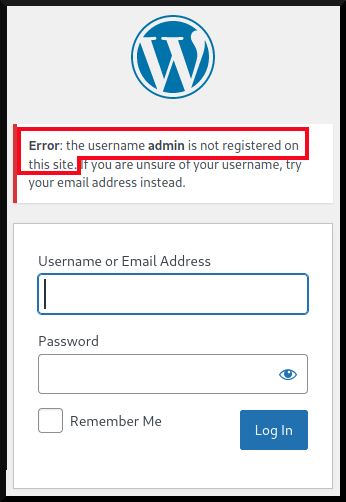
\includegraphics[width=0.50\textwidth]{14-wp-login-admin.png}
        \caption{Checking the existence of the user \textbf{admin}}
    \end{figure}

    \textit{WordPress} warns us that this user, \textbf{admin}, doesn't exist.
    Let's check the username found on the blog post:

    \begin{figure}[H]\label{pic:15-wp-login-albert}
        \centering
        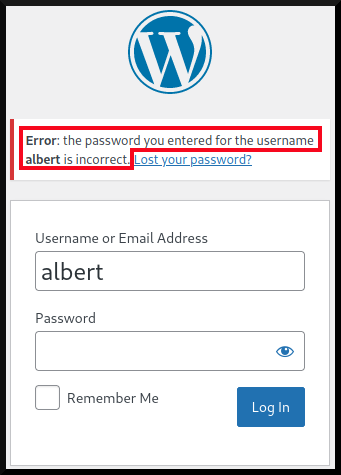
\includegraphics[width=0.50\textwidth]{15-wp-login-albert.png}
        \caption{Checking the existence of the user \textbf{albert}}
    \end{figure}

    The message got is completely different from the previous one. This tells
    us the password is incorrect, but the user exists! However, we don't have a
    clue of what the password is, and as brute force is the last thing we
    should apply, let's look up on the Internet what \textbf{symposium} is.

    \textbf{wp-symposium} is a \textit{WordPress} plugin, let's see if it has
    known vulnerabilities:

    \begin{figure}[H]\label{pic:16-searchsploit-symposium}
        \centering
        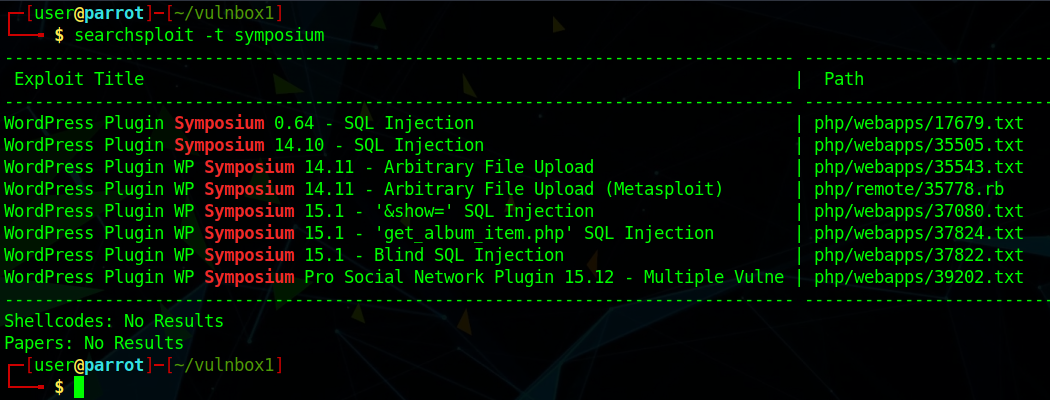
\includegraphics[width=1.00\textwidth]{16-searchsploit-symposium.png}
        \caption{Looking for known \textbf{symposium} vulnerabilities}
    \end{figure}

    There are quite a few of vulnerabilities. We don't know how useful they are
    until we know the version. Looking for its source code on \textit{GitHub}:

    \begin{figure}[H]\label{pic:17-ddg-symposium-github}
        \centering
        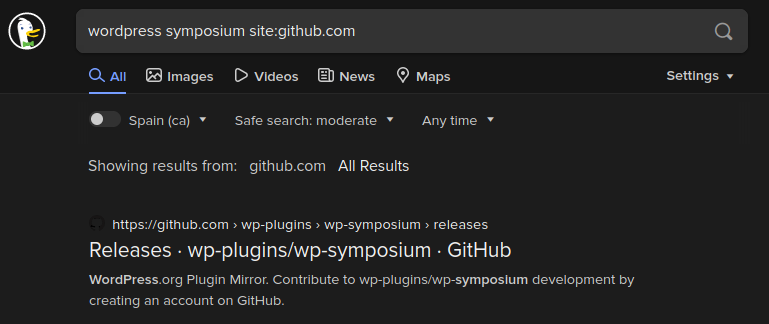
\includegraphics[width=1.00\textwidth]{17-ddg-symposium-github.png}
        \caption{Looking up for \textbf{symposium} source code}
    \end{figure}

    I decided to download the latest version to see where I can get information
    about the version:

    \begin{figure}[H]\label{pic:18-github-wp-symposium}
        \centering
        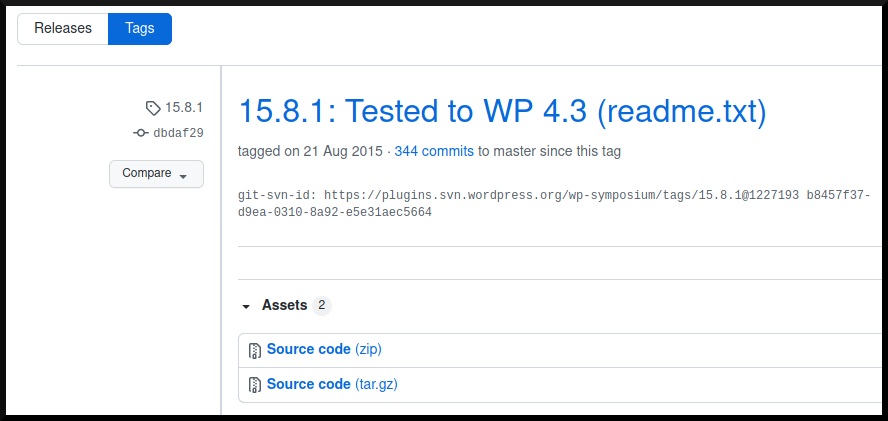
\includegraphics[width=1.00\textwidth]{18-github-wp-symposium.png}
        \caption{Downloading \textbf{wp-symposium} source code}
    \end{figure}

    We can download the source code and seek for patterns, like
    \textit{version} or common files where the version might be, like
    \textit{changelog} or \textit{readme}, and so on:

    \begin{figure}[H]\label{pic:19-src-symposium}
        \centering
        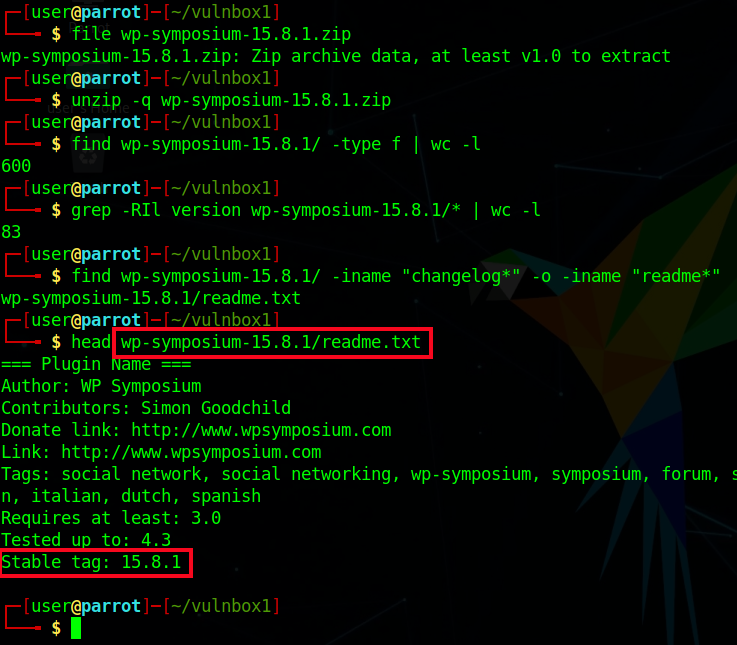
\includegraphics[width=1.00\textwidth]{19-src-symposium-gimp.png}
        \caption{Looking for what file may contain the version}
    \end{figure}

    As we can see, there are 600 files, 83 of them have the word
    \textit{version}. It's quite a lot.
    Searching only for some common files we can find \textbf{readme.txt} and
    within its first ten lines we see the version: \textit{15.8.1}

    We know that's the version because it's the one we've downloaded.

    Now we know what file to aim in order to get the version and see whether or
    not is vulnerable.

    \textit{WordPress} stores its plugins on 
    \verb!{WORDPRESS}/wp-content/plugins/!, we should see if we can reach this
    path on the remote system:

    \begin{figure}[H]\label{pic:20-curl-symposium-check}
        \centering
        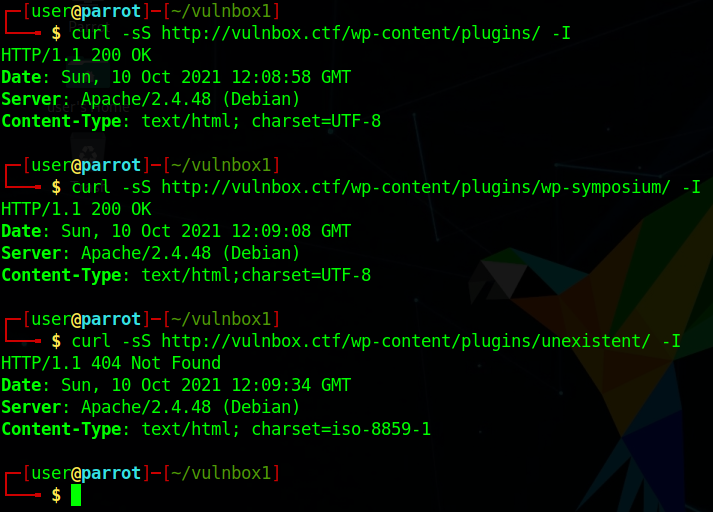
\includegraphics[width=1.00\textwidth]{20-curl-symposium-check.png}
        \caption{Checking for the existence of \textbf{wp-symposium} path}
    \end{figure}

    We see we can reach both the plugins path and the \textbf{wp-symposium}
    location\footnote{They both return a \textbf{200 OK} HTTP response code.},
    and if we try to get another path, like \textit{unexistent} we get the
    infamous \textit{404 Not Found} response.

    Let's see if the \textbf{readme.txt} file is present:

    \begin{figure}[H]\label{pic:21-curl-symposium-version}
        \centering
        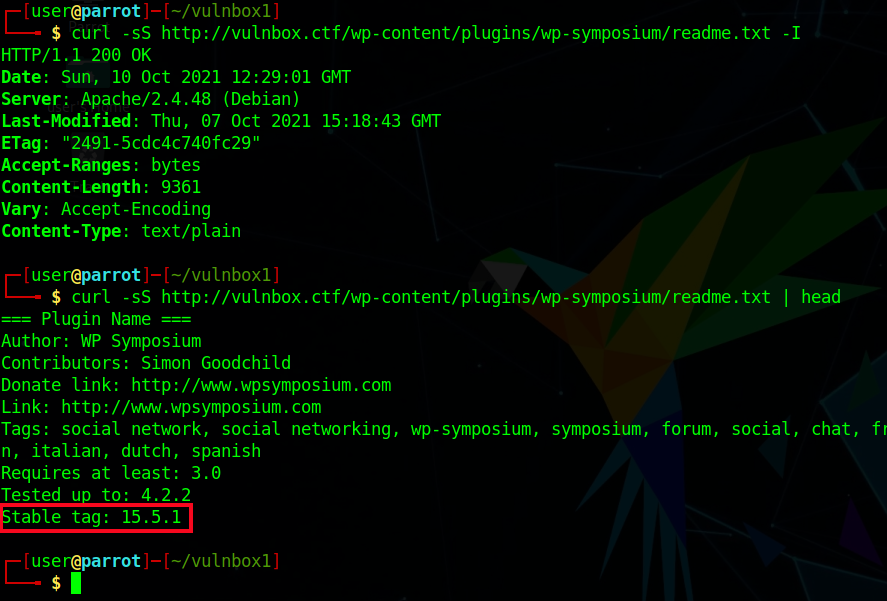
\includegraphics[width=1.00\textwidth]{21-curl-symposium-version-gimp.png}
        \caption{Discovering our target's \textbf{symposium} version}
    \end{figure}

    Not only does it exist, but it also gives us the current version installed,
    as expected.

    Going back to the results of \texttt{searchsploit} we have at least three
    possible exploits to test. I'll try the second one. We should mirror it to
    get it into our current working directory:

    \begin{figure}[H]\label{pic:22-searchsploit-mirror}
        \centering
        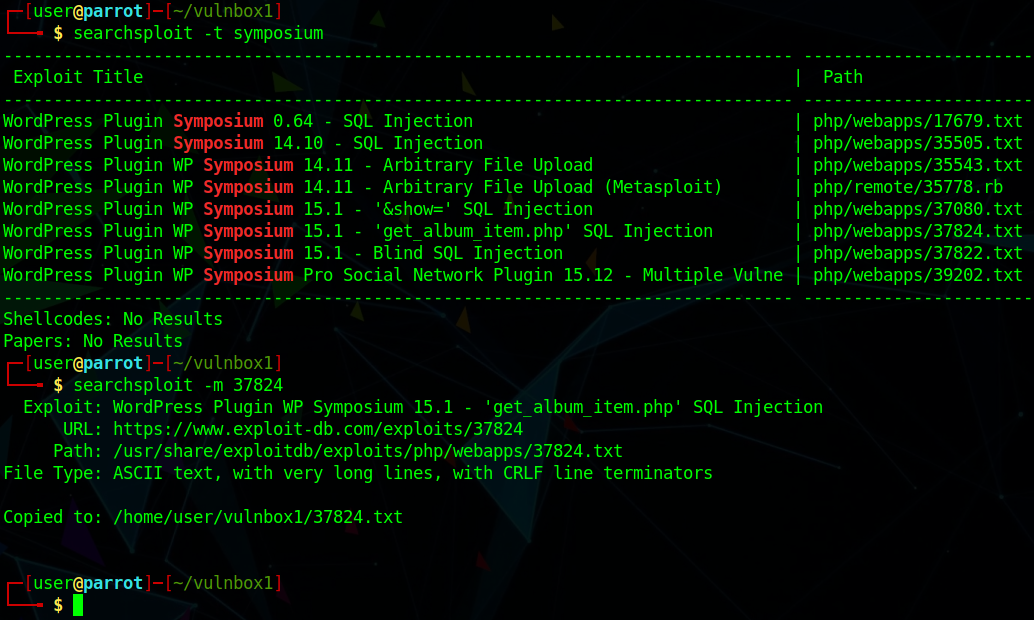
\includegraphics[width=1.00\textwidth]{22-searchsploit-mirror.png}
        \caption{Mirroring the exploit}
    \end{figure}

    Read it, and get the part we need the most, the exploitation one:

    \begin{figure}[H]\label{pic:23-grep-PoC}
        \centering
        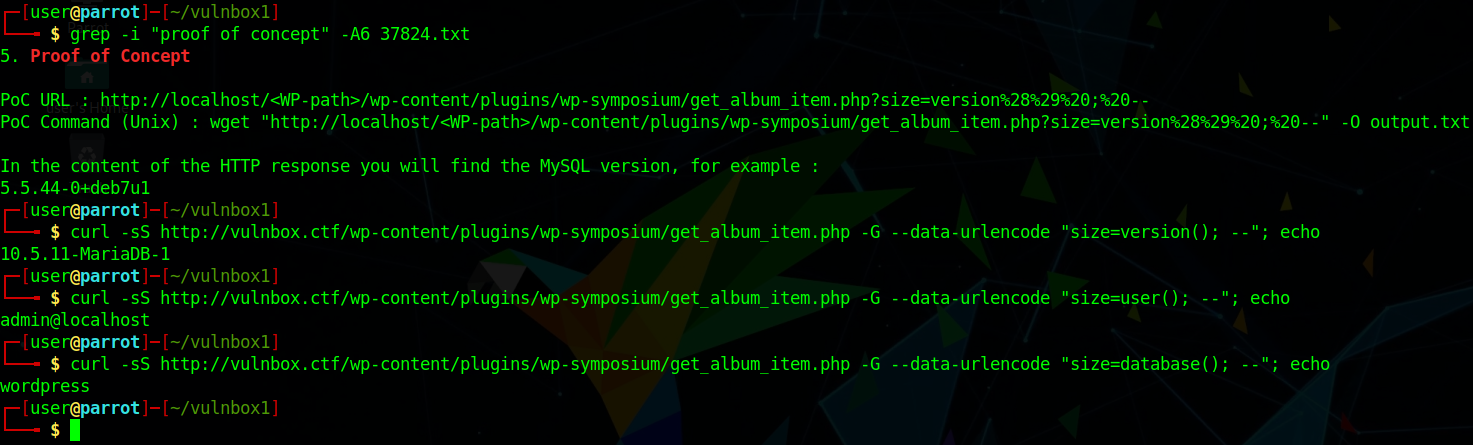
\includegraphics[width=1.00\textwidth]{23-grep-PoC.png}
        \caption{Testing the \textit{PoC}}
    \end{figure}

    It works just fine!

    Writing that query is quite time consuming, modifying it is a little
    cumbersome and error prone. It's better if we write our own exploit:

    \begin{figure}[H]\label{pic:24-batcat-exploit}
        \centering
        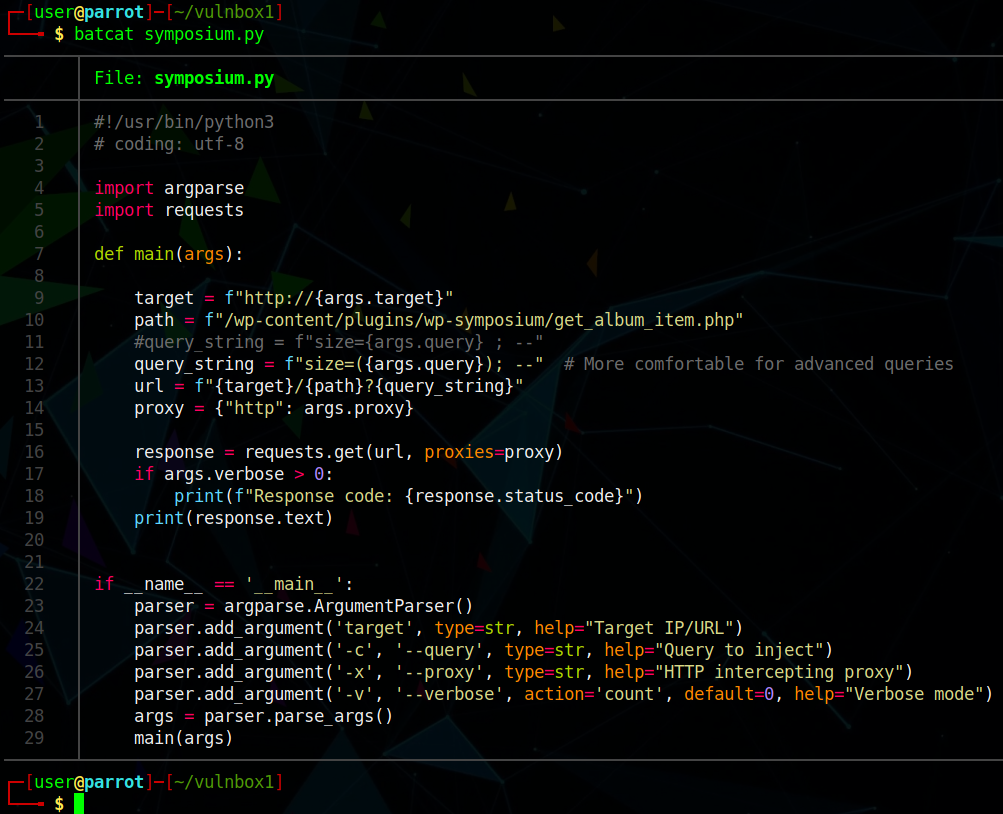
\includegraphics[width=1.00\textwidth]{24-batcat-exploit.png}
        \caption{Exploit written in \textit{Python}}
    \end{figure}

    We must test it:

    \begin{figure}[H]\label{pic:25-exploit-basic-info}
        \centering
        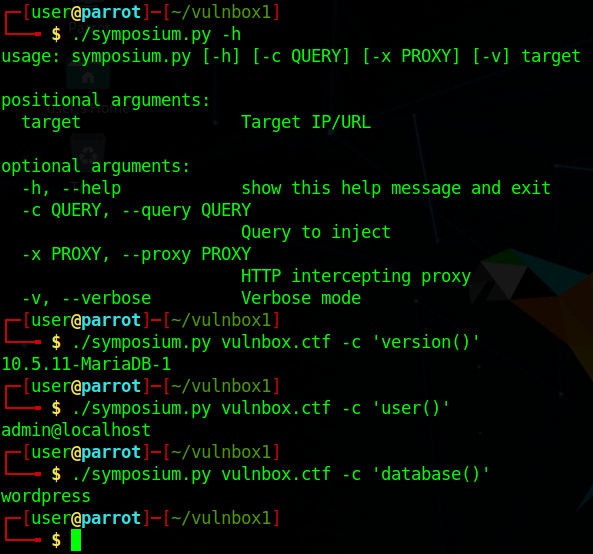
\includegraphics[width=1.00\textwidth]{25-exploit-basic-info.png}
        \caption{Testing the exploit}
    \end{figure}

    It seems to work right. Let's enumerate the databases:

    \begin{figure}[H]\label{pic:26-exploit-databases}
        \centering
        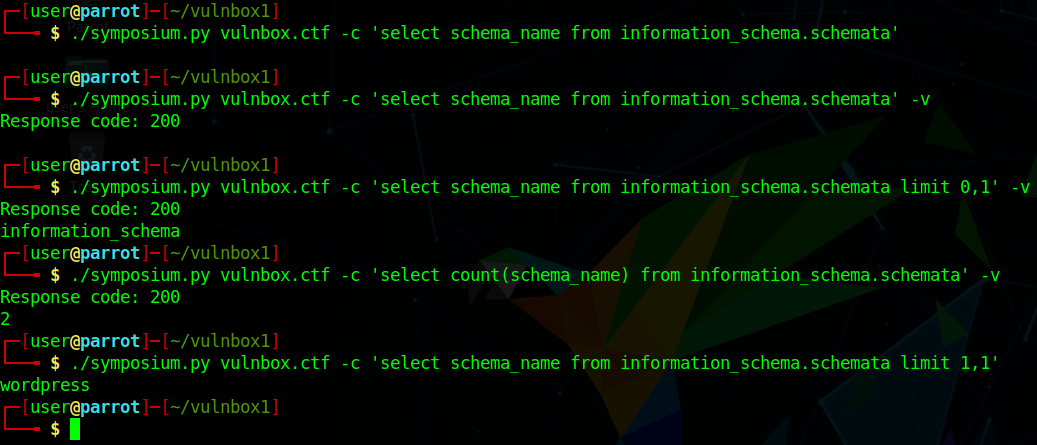
\includegraphics[width=1.00\textwidth]{26-exploit-databases.png}
        \caption{Enumerating databases}
    \end{figure}

    I'd like to break down the process I've made here:
    \begin{enumerate}
        \item I try to get the databases from
            \textbf{information\_schema.schemata}.
        \item As I don't get any output, I try to see the response code.
        \item As the response code seems to have fetched an empty page, it
            might have happened because the query can't return more than one
            result at a time. So I limit the number of results to 1.
        \item Since it worked, we are shown the first database from the output,
            I want to know how many of them there are by counting them.
        \item There are only two databases, so I only try to get the next one:
            \textbf{wordpress}.
    \end{enumerate}

    The important data is actually on the \textbf{wordpress} database, we're 
    using \textbf{information\_schema} to get information about the schemas and
    their structure.

    Let's try to get the tables from our target database:

    \begin{figure}[H]\label{pic:27-exploit-tables-1}
        \centering
        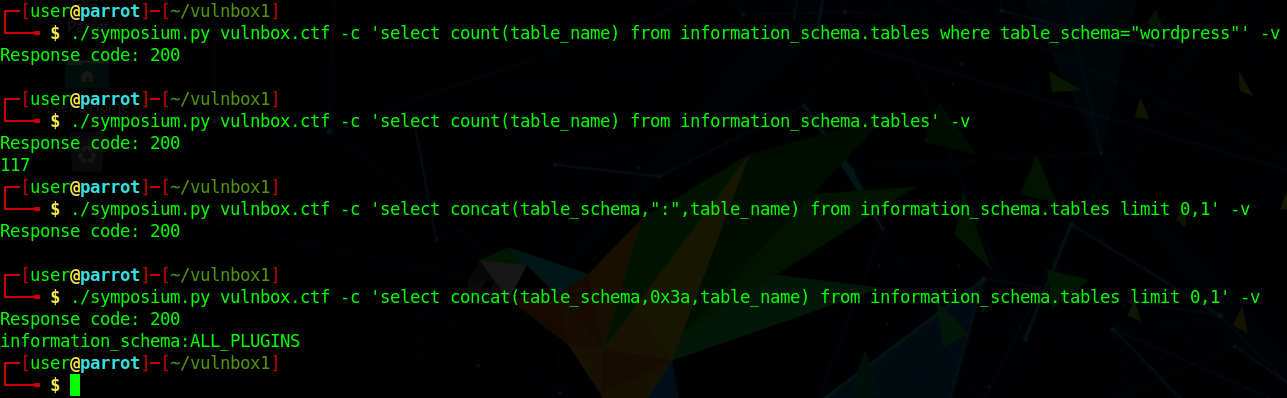
\includegraphics[width=1.00\textwidth]{27-exploit-tables-1.png}
        \caption{Enumerating tables: a first approach}
    \end{figure}

    \begin{enumerate}
        \item I try to retrieve the tables in the \textbf{wordpress} database.
            But I get an empty response instead.
        \item I remove the \texttt{where} clause to see if there's any problem
            with the filtering. And I receive the amount of tables on the whole
            DBMS.
        \item As I won't able to tell which tables belong to which database, I
            decide to concatenate the database along with the table name.
            Separated by a colon. It didn't work though.
        \item The \texttt{concat} function should exist, and as the filtering
            clause hadn't worked either, that makes me think there's a problem
            with the double quotes\footnote{The same happen if we try with
            single quotes.}.
            \newline
            I then use the colon's hexadecimal representation (\texttt{0x3a})
            and it worked!
    \end{enumerate}

    There are two approaches I can think of right now to enumerate the tables.
    The first of them is to do exactly what we have just done and filtering
    with \texttt{grep} to get solely the tables in the \textbf{wordpress}
    database, like this:

    \begin{figure}[H]\label{pic:28-exploit-tables-2}
        \centering
        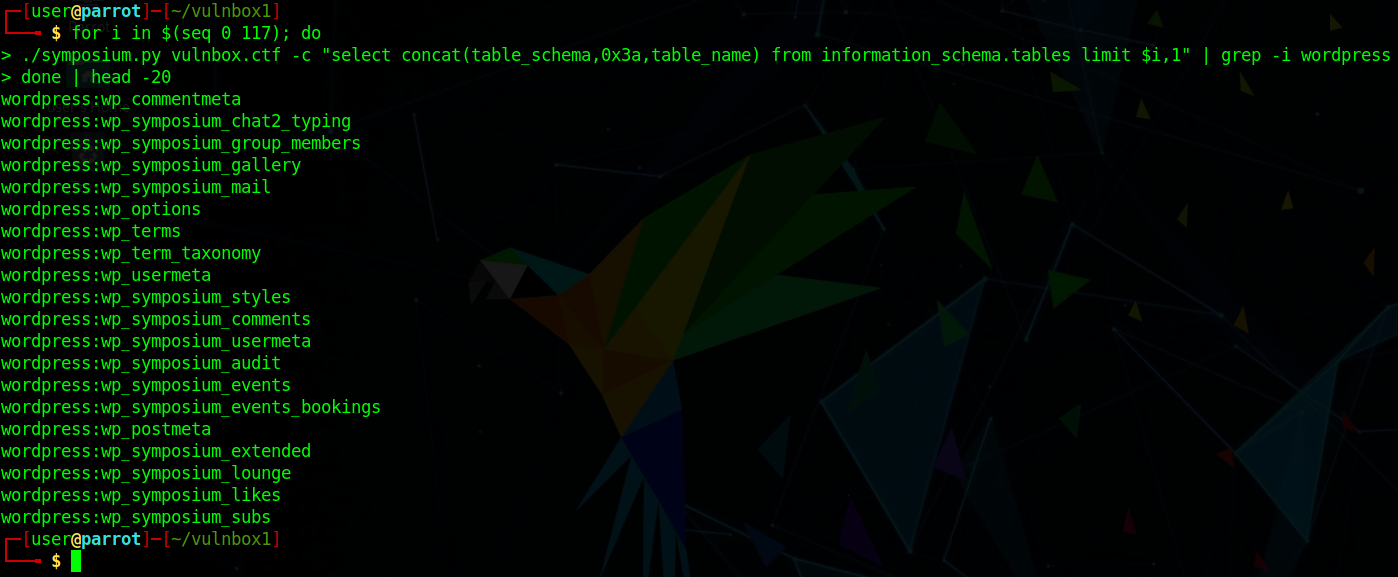
\includegraphics[width=1.00\textwidth]{28-exploit-tables-2.png}
        \caption{Enumerating tables: getting the tables the slow way}
    \end{figure}

    It works! But the output is kind of slow, as it has to make 118 
    requests\footnote{from 0 to 117, this last response should be empty} and
    filter the ones we're interested in.

    The thing is, we know what the issue with the queries was: the quotes!
    And we know we can bypass it using hexadecimal, as we've proved with
    \texttt{0x3a}.

    Let's try to do the same with the database name:

    \begin{figure}[H]\label{pic:29-exploit-tables-3}
        \centering
        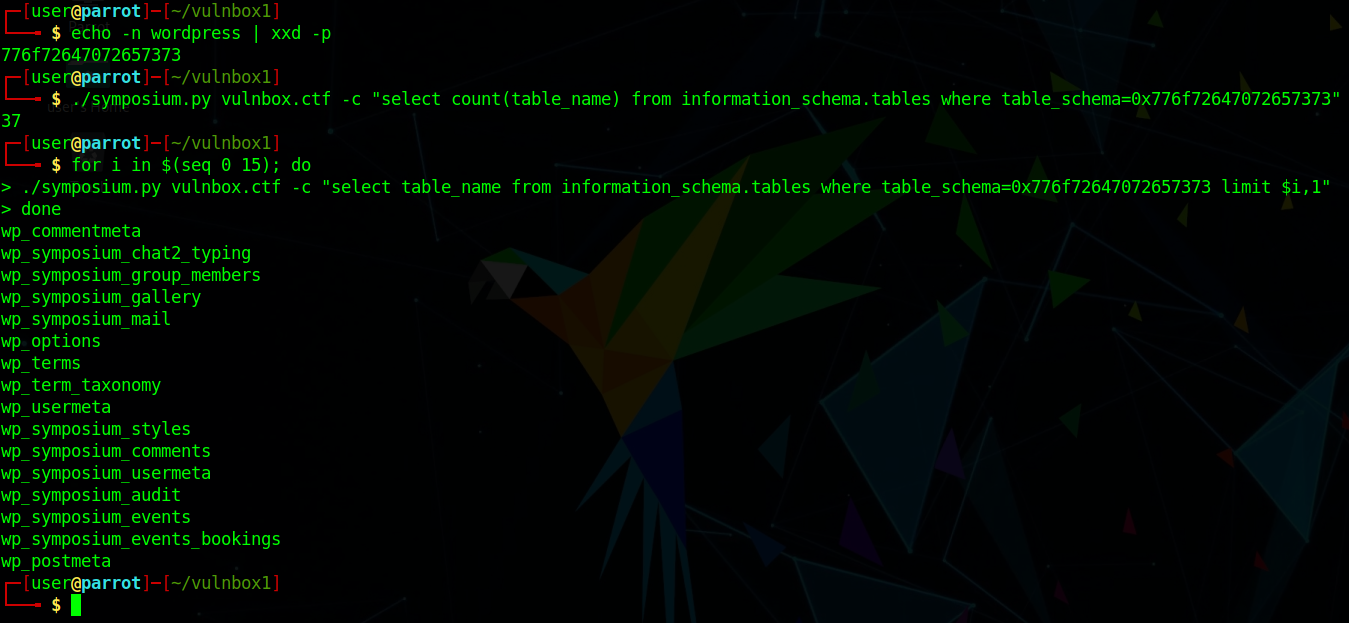
\includegraphics[width=1.00\textwidth]{29-exploit-tables-3.png}
        \caption{Enumerating tables: getting the tables, a better way}
    \end{figure}

    \begin{enumerate}
        \item I see the hexadecimal representation of the word
            \textbf{wordpress}. Note I've removed the line feed with the option
            \texttt{-n}.
        \item I tested to see if it worked and it did indeed!
        \item We can now retrieve the table names in a more comfortable and
            quick way. Note I have requested for the first 16 ones, just to
            show how it worked and not to have a huge output.
    \end{enumerate}

    If we performed the previous command with \verb!seq 0 37! we would get all
    the table names we were aiming.

    We're specially interested in credentials, therefore the table
    \textbf{wp\_users}\footnote{This table isn't shown in the screenshot but we
    can get it when getting all the tables.} catches our eye.

    We can get the columns from \textbf{wp\_users} filtering by both the
    database and table:

    \begin{figure}[H]\label{pic:30-exploit-columns}
        \centering
        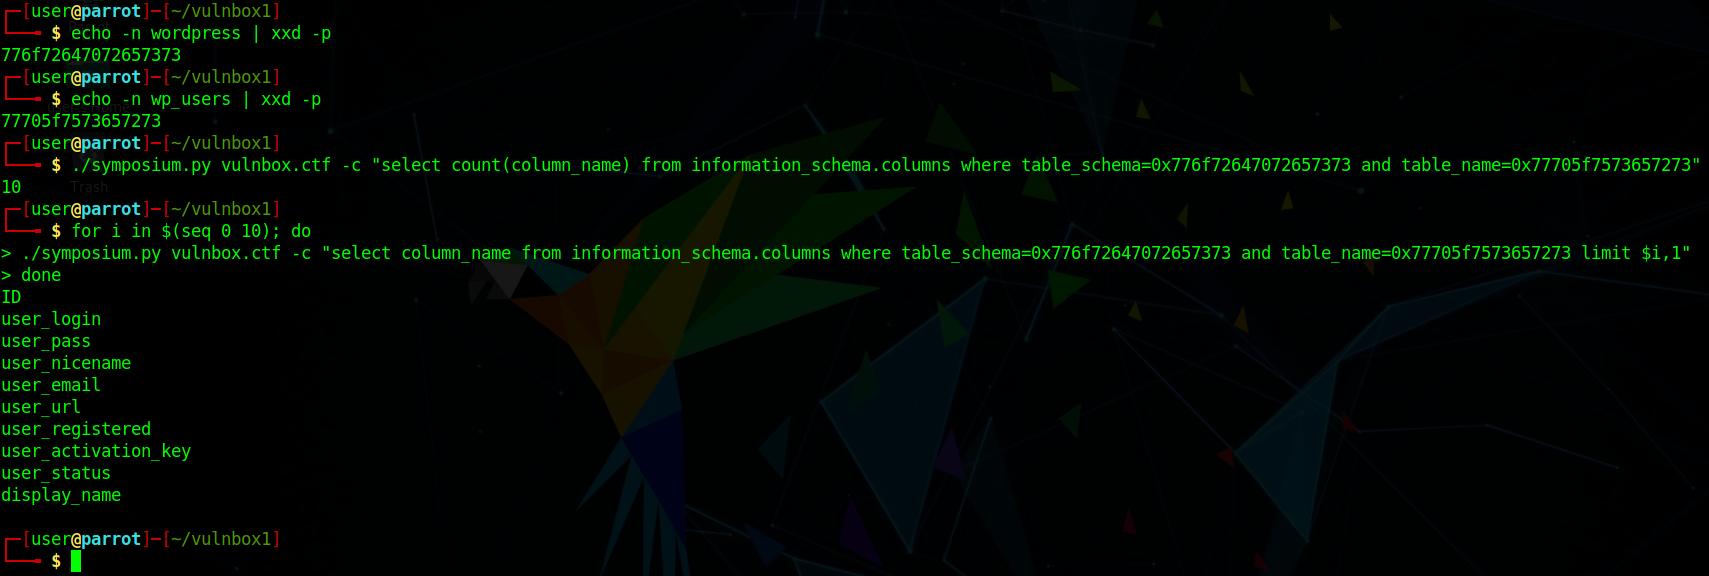
\includegraphics[width=1.00\textwidth]{30-exploit-columns.png}
        \caption{Enumerating columns from \textbf{wp\_users}}
    \end{figure}

    Getting the table contents now is trivial. Let's get what we are interested
    in: \textbf{user\_login} and \textbf{user\_pass}

    \begin{figure}[H]\label{pic:31-exploit-users}
        \centering
        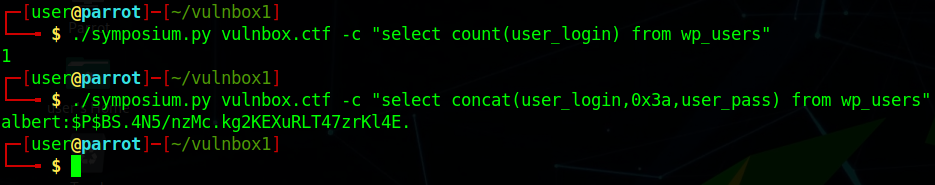
\includegraphics[width=1.00\textwidth]{31-exploit-users.png}
        \caption{Getting credentials from \textbf{wp\_users}}
    \end{figure}

    As the \textbf{user\_pass} is likely to be hashed, let's try to break it
    with \texttt{john}:

    \begin{figure}[H]\label{pic:32-john-wordpress}
        \centering
        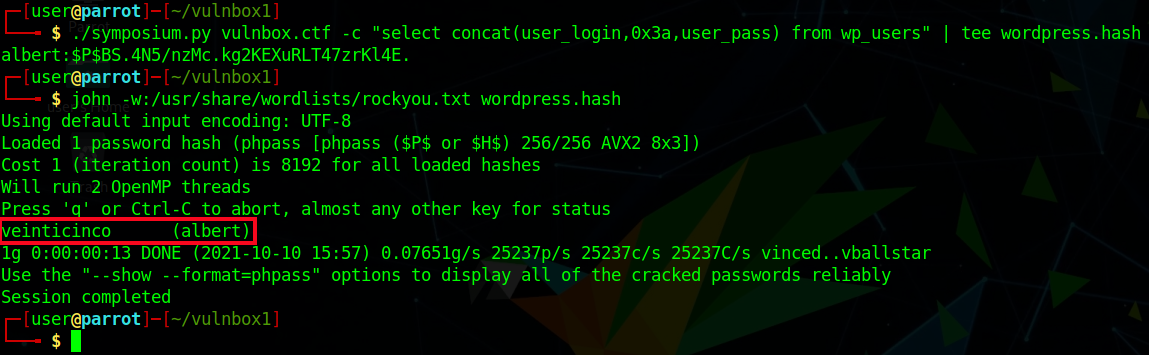
\includegraphics[width=1.00\textwidth]{32-john-wordpress-gimp.png}
        \caption{Cracking \textit{WordPress} credentials}
    \end{figure}

\pagebreak
\subsubsection{Gaining Access}

    With the credentials gathered:

    \verb!albert:veinticinco!

    we can access the CMS as administrator:

    \begin{figure}[H]\label{pic:33-wp-albert}
        \centering
        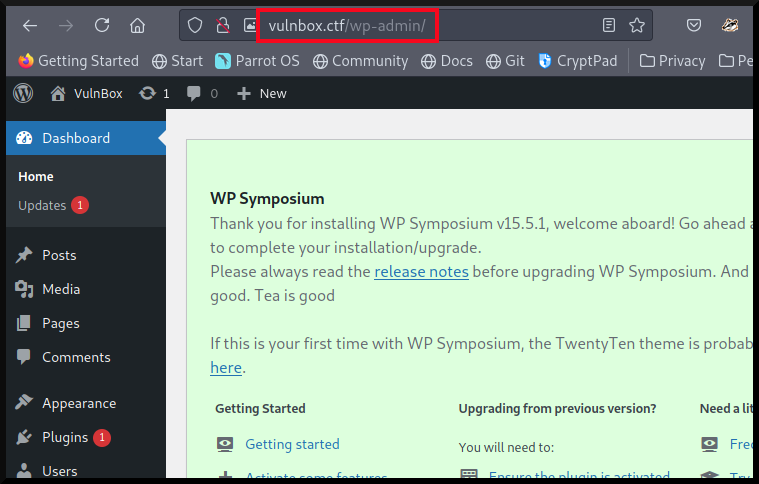
\includegraphics[width=1.00\textwidth]{33-wp-albert.png}
        \caption{\textit{WordPress} admin panel}
    \end{figure}

    To gain access to the system we can try the usual way: modifying the theme.

    Let's go to \textbf{Appearance} $\rightarrow$ \textbf{Theme Editor}

    \begin{figure}[H]\label{pic:34-wp-theme-editor}
        \centering
        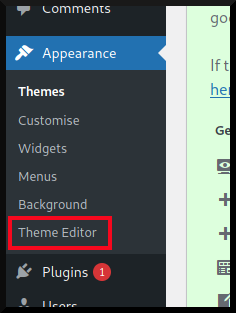
\includegraphics[width=0.45\textwidth]{34-wp-theme-editor.png}
    \end{figure}

    The common template we use is the \texttt{404.php}, we have to take into
    account what theme we're modifying, in our case is the
    \textbf{twentytwentyone}, the active one\footnote{There are three themes in
    this \textit{WordPress}: \textbf{twentynineteen}, \textbf{twentytwenty} and
    \textbf{twentytwentyone}. All of them have similar structures, and we can
    use any of them regardless of whether or not is active.}, it's important to
    know this because we are going to run system commands through the
    \textit{webshell} by specifying the path and a query string.

    \begin{figure}[H]\label{pic:35-wp-webshell}
        \centering
        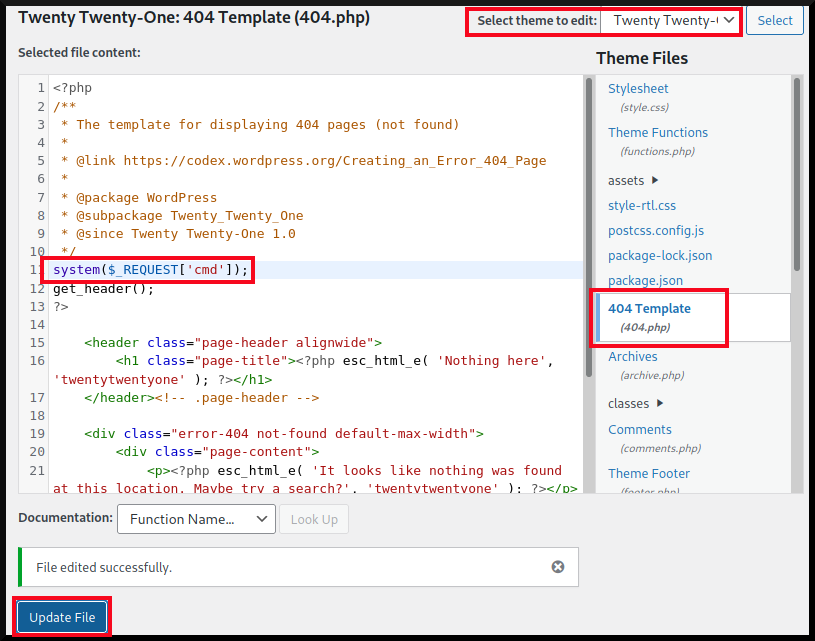
\includegraphics[width=1.00\textwidth]{35-wp-webshell-gimp.png}
        \caption{Setting a \textit{Webshell}}
    \end{figure}

    Once updated successfully, we ought to test its functionality:

    \begin{figure}[H]\label{pic:36-curl-rce-test}
        \centering
        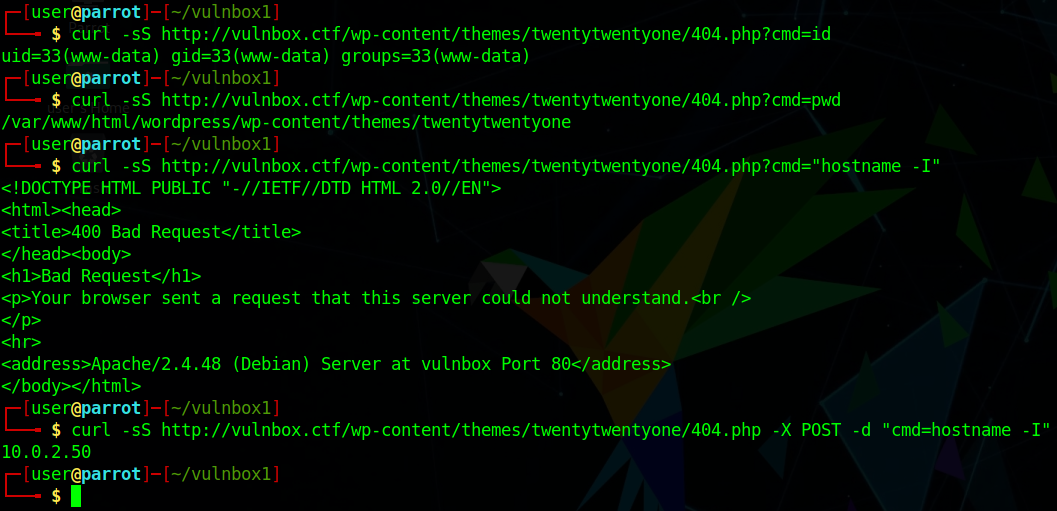
\includegraphics[width=1.00\textwidth]{36-curl-rce-test.png}
        \caption{Testing our \textit{webshell}}
    \end{figure}

    We've got \textbf{RCE}!

    Note I'm able to run commands with both \textbf{GET} and \textbf{POST}
    requests, due to \verb!$_REQUEST['cmd']!. If I had used \verb!$_GET['cmd']!
    I would only be able to make \textbf{GET} requests, likewise with
    \verb!$_POST['cmd']! I'd only be able to make \textbf{POST} requests.

    The next step is to get a shell to get into the system.

    There are a number of tools and techniques we can use to achieve this, the
    most well-known is \texttt{netcat}, even though, it's installed in the
    system we'll be leveraging the one it's install for sure: \texttt{bash}.

    \begin{figure}[H]\label{pic:37-reverse-shell}
        \centering
        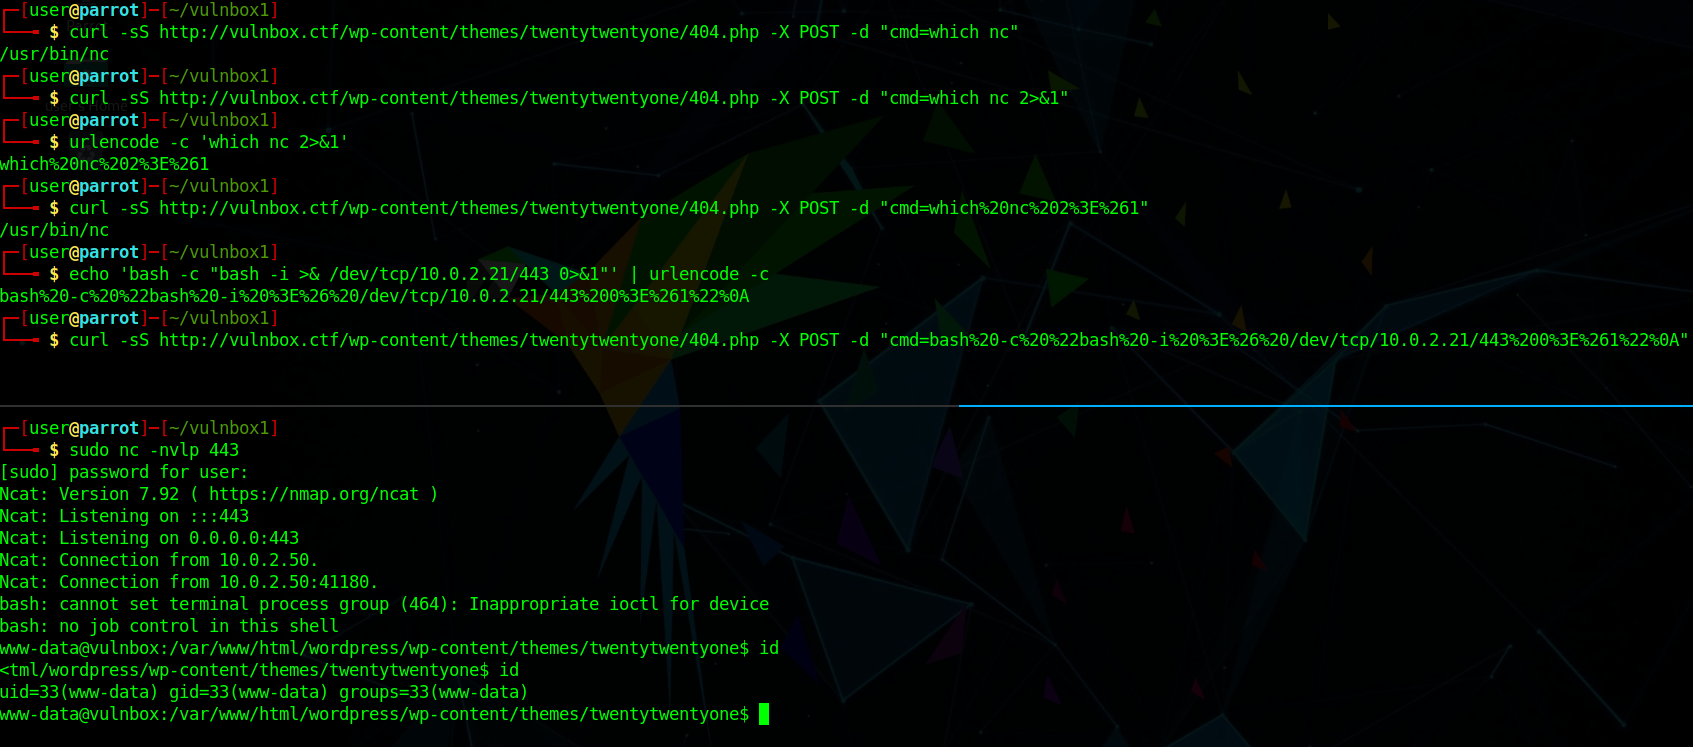
\includegraphics[width=1.00\textwidth]{37-reverse-shell.png}
        \caption{Getting a \textit{reverse shell}}
    \end{figure}

    \begin{enumerate}
        \item We check for the existence of \texttt{netcat}, and it's
            installed\footnote{Even though it's installed, the version may not
            support the \texttt{-e} or \texttt{-c} options, which run a command
            on the destination.}
        \item As we know we have a positive output from the previous command,
            we may try to do it again redirecting the \textbf{stderr} to
            \textbf{stdout}, this should make no difference, but it does. The
            reason is because the ampersand (\verb!&!) is used to separate
            parameters, and this request raises an error and we receive no
            output at all.
        \item To overcome this issue, we have to encode the parameter in
            \textbf{URL format}\footnote{The tool I'm using I created myself,
            you won't find it on your system. You can encode it in other ways,
            like searching a web page for this purpose, or use \textbf{python},
            or \textbf{php} among others.}
            You can also do this with\newline
            \verb!php -r "echo urlencode('which nc 2>&1');"!.
        \item Once we know the parameters encoded work, we can try to establish
            a reverse shell.
    \end{enumerate}

    As we can see, we've got a reverse shell, to work more comfortable, we
    should upgraded:

    \begin{figure}[H]\label{pic:38-upgrading-shell}
        \centering
        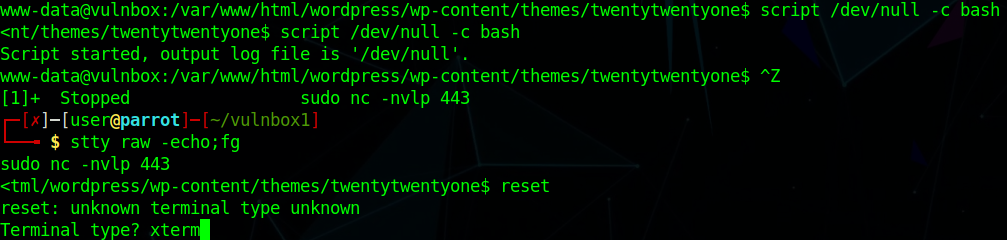
\includegraphics[width=1.00\textwidth]{38-upgrading-shell.png}
        \caption{Upgrading the shell}
    \end{figure}

    The steps I make are:

    \begin{enumerate}
        \item \verb!script /dev/null -c bash!
        \item I stop the current session with \textbf{Ctrl+Z}.
        \item \verb!stty raw -echo; fg!
        \item \verb!reset!
        \item The prompt asks for the type of shell, even when we specify it,
            it won't set that value. So we have to do it ourselves.
        \item \verb!export TERM=xterm!
        \item \verb!export SHELL=bash!
        \item \verb!stty rows 39 columns 191!\footnote{This is the size of my
            console, but it may be different in your case, try \texttt{stty size}
            within another console to take the values from.}
    \end{enumerate}

    \begin{figure}[H]\label{pic:39-fully-upgraded-shell}
        \centering
        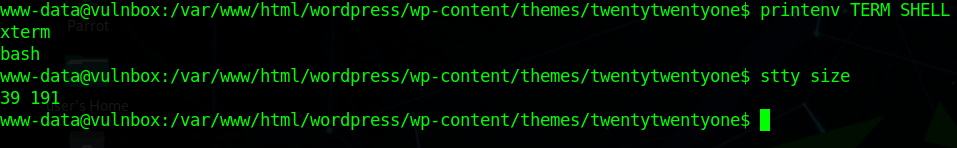
\includegraphics[width=1.00\textwidth]{39-fully-upgraded-shell.png}
        \caption{Shell upgraded}
    \end{figure}

\pagebreak
\subsubsection{Lateral Movement: albert}

    Let's enumerate the users on the machine to know which ones could be our
    main targets, apart from \textbf{root}, of course:

    \begin{figure}[H]\label{pic:40-enumerating-users}
        \centering
        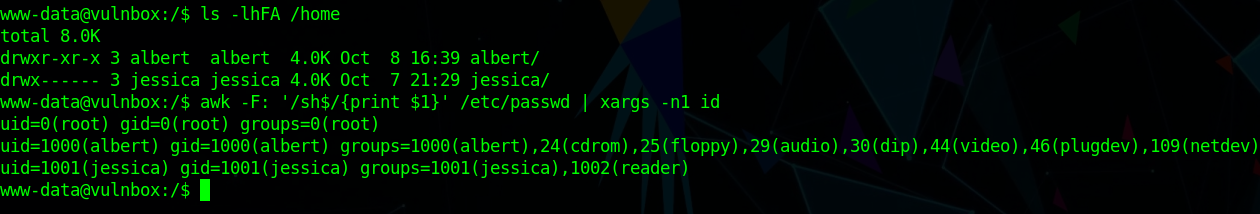
\includegraphics[width=1.00\textwidth]{40-enumerating-users.png}
        \caption{Enumerating system users}
    \end{figure}

    With this information the user \textbf{albert} seems to be our main target,
    as he's on more groups and \textbf{jessica} doesn't seem to be in an
    important group.

    On the other hand, \textbf{jessica}'s permissions to her home directory
    are more restrictive and it would be harder to get more information than
    with \textbf{albert}.

    \begin{figure}[H]\label{pic:41-albert-home}
        \centering
        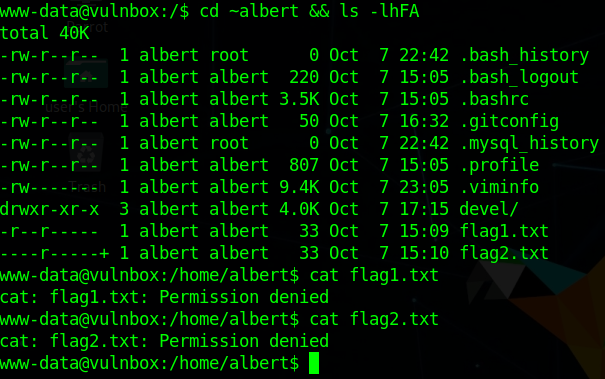
\includegraphics[width=0.85\textwidth]{41-albert-home.png}
        \caption{\textbf{albert}'s home directory's contents}
    \end{figure}

    We can't read neither \texttt{flag1.txt} nor \texttt{flag2.txt}. Both
    \texttt{.bash\_history} and \texttt{.mysql\_history} are empty. Let's see
    what's in \texttt{devel}:

    \begin{figure}[H]\label{pic:42-devel-contents}
        \centering
        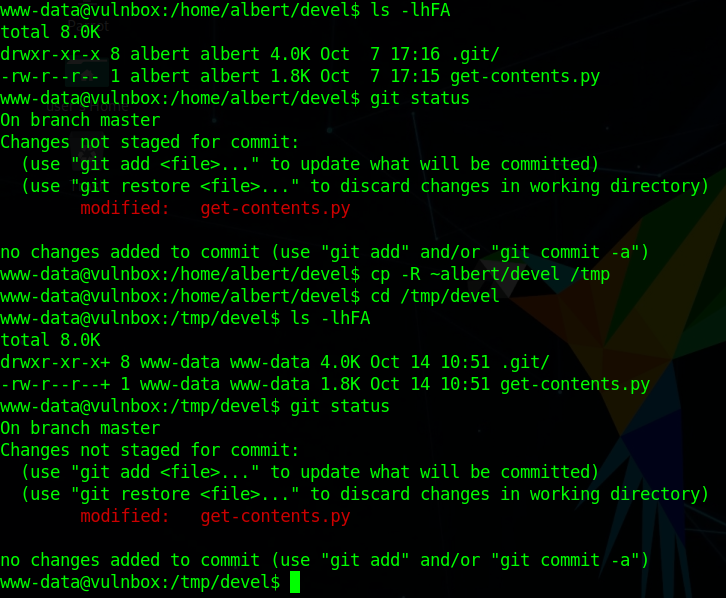
\includegraphics[width=1.00\textwidth]{42-devel-contents.png}
        \caption{\texttt{devel} folder contents}
    \end{figure}

    It's a project versioned with \texttt{git}. If we run \verb!git status! we
    can see there are changes from the previous commit. There's nothing
    interesting in the python script we can see.

    As we don't have write permissions we won't be able to go to previous
    commits. So, we should copy the whole project to where we can do it, like
    \texttt{/tmp}, and make sure we've copied everything exactly as it is.

    To see what are the differences between the current script and the previous
    version, we can issue \verb!git diff get-contents.py!. But, once again, we
    don't get anything interesting. Maybe there were other files removed or
    more branches.

    \begin{figure}[H]\label{pic:43-git-branch}
        \centering
        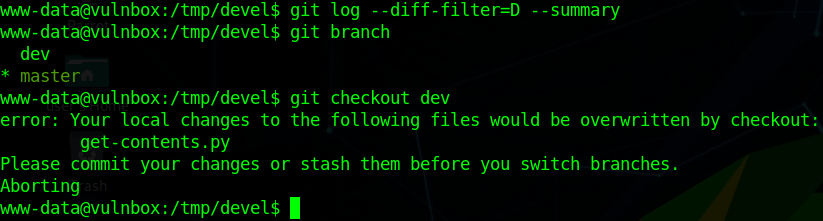
\includegraphics[width=1.00\textwidth]{43-git-branch.png}
        \caption{Looking for deleted items and more branches}
    \end{figure}

    Filtering by deleted files/folders, we don't get anything. Checking for the
    existence of more branches, we find out the \textbf{dev} branch. But we
    can't switch to it because our current branch, \textbf{master}, has
    uncommitted changes.

    With \texttt{git status} we could also see there were files which weren't
    added for the commit, so we should add them and then make the commit:

    \begin{figure}[H]\label{pic:44-git-checkout-dev}
        \centering
        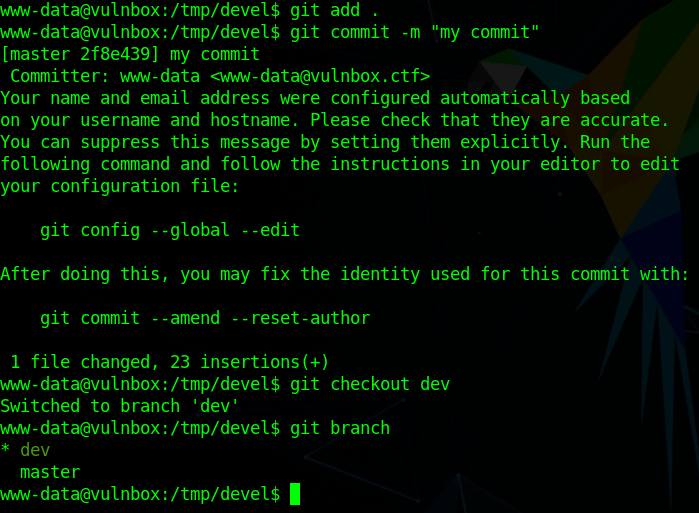
\includegraphics[width=1.00\textwidth]{44-git-checkout-dev.png}
        \caption{Committing and moving to \textbf{dev} branch}
    \end{figure}

    And we're in \textbf{dev} branch now. If we see the contents, there's a new
    file, namely \texttt{jessica.txt}:

    \begin{figure}[H]\label{pic:45-cat-jessica}
        \centering
        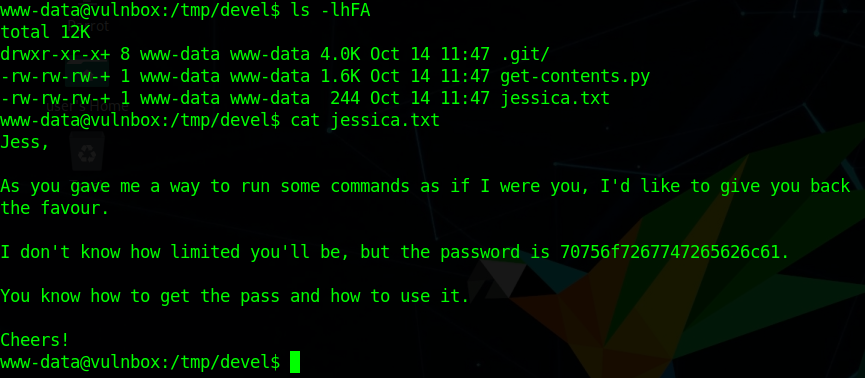
\includegraphics[width=1.00\textwidth]{45-cat-jessica.png}
        \caption{Reading \texttt{jessica.txt}}
    \end{figure}

    As we can read, we have a password in hexadecimal which \textbf{albert} is 
    providing to \textbf{jessica}, then we try to log in with this to 
    \textbf{albert}, but it fails. Although it makes little sense, we have to 
    try with every single user (\textit{password spraying}). We don't succeed.

    If we reverse the password found, we see a hint: \textit{albertgroup}:

    \begin{figure}[H]\label{pic:46-xxd-password}
        \centering
        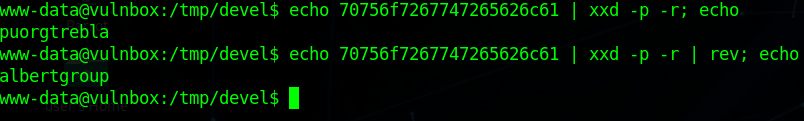
\includegraphics[width=1.00\textwidth]{46-xxd-password.png}
        \caption{Revealing the password and the hint}
    \end{figure}

    We may already know we can start a shell with another user, as long as we
    know the password, with \verb!su - <user>!, but we can do the same with a
    group! It has to have a password assigned though:

    \begin{figure}[H]\label{pic:47-flag1}
        \centering
        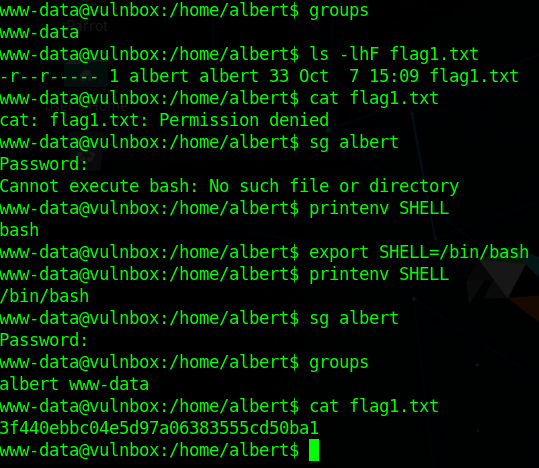
\includegraphics[width=1.00\textwidth]{47-flag1.png}
        \caption{Changing groups and reading \texttt{flag1.txt}}
    \end{figure}

    \begin{itemize}
        \item With \verb!groups! we list the groups we belong to.
        \item With \verb!sg <group>! we can add ourselves to another group.
        \item \verb!printenv <variable>! prints exported environmental variables.
    \end{itemize}

    We had a problem trying to get into \textbf{albert} group because it didn't
    find the \textit{shell} specified. It needed the full path to it, once
    provided we got into our target group and could read the first flag.

    Nevertheless, we can't read \texttt{flag2.txt}, even though we are in the
    group \textbf{albert}:

    \begin{figure}[H]\label{pic:48-cat-flag2-forbidden}
        \centering
        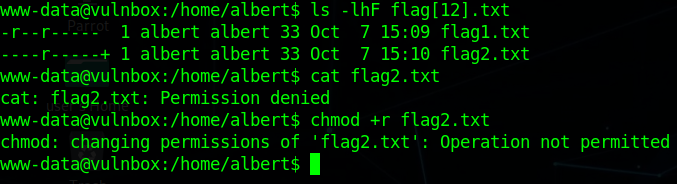
\includegraphics[width=1.00\textwidth]{48-cat-flag2-forbidden.png}
        \caption{We can't read or change \texttt{flag2.txt} permissions}
    \end{figure}

    Neither can we change its permissions.

    Inspecting the file further, we were able to see a plus sign within the
    permissions. This indicates it has \textbf{ACL}s\footnote{\textbf{ACL}:
    \textit{Access Control Lists}}, let's see them:

    \begin{figure}[H]\label{pic:50-getfacl}
        \centering
        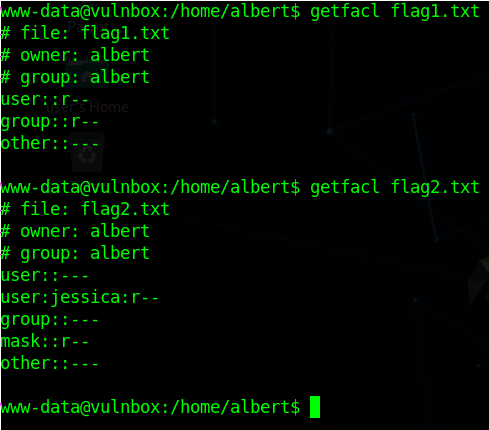
\includegraphics[width=0.80\textwidth]{50-getfacl.png}
        \caption{Listing the \textbf{ACL}s of \texttt{flag2.txt}}
    \end{figure}

    It seems neither \textbf{albert} is able to read the file, unless he
    changes the permissions as he's the owner, but \textbf{jessica} can.

\pagebreak
\subsubsection{Lateral Movement: jessica}

    Enumerating schedule tasks (\textbf{cronjobs}), we have an interesting
    finding:

    \begin{figure}[H]\label{pic:51-enumerating-cronjobs}
        \centering
        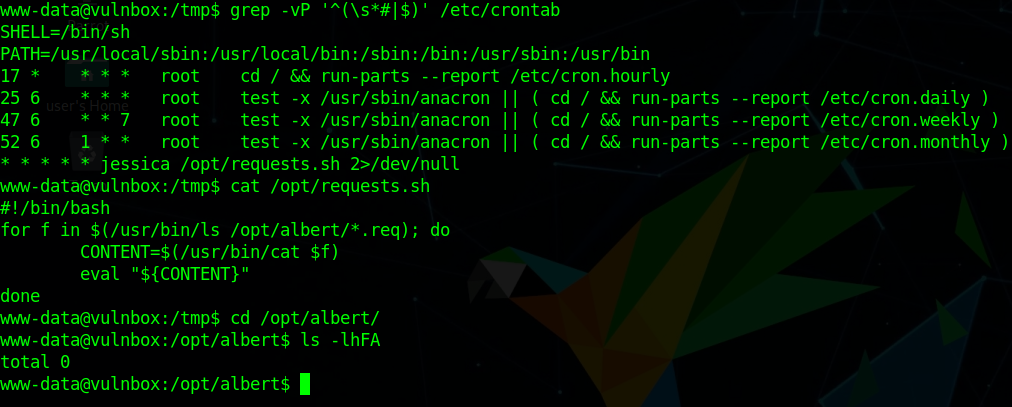
\includegraphics[width=1.00\textwidth]{51-enumerating-cronjobs.png}
        \caption{\textbf{cronjobs} enumerating with finding}
    \end{figure}

    The last line of \texttt{/etc/crontab} tells us the script
    \texttt{/opt/requests.sh} is being run by \textbf{jessica} every minute.

    The contents of the previous script shows how any file within
    \verb!/opt/albert! with the extension \verb!.req! is being executed.

    And this folder is empty. As we don't know what is inside
    \textbf{jessica}'s home folder, we can start by enumerating its contents,
    or starting with something easier, reading \texttt{flag2.txt}:

    \begin{figure}[H]\label{pic:52-cronjob-cat-flag2}
        \centering
        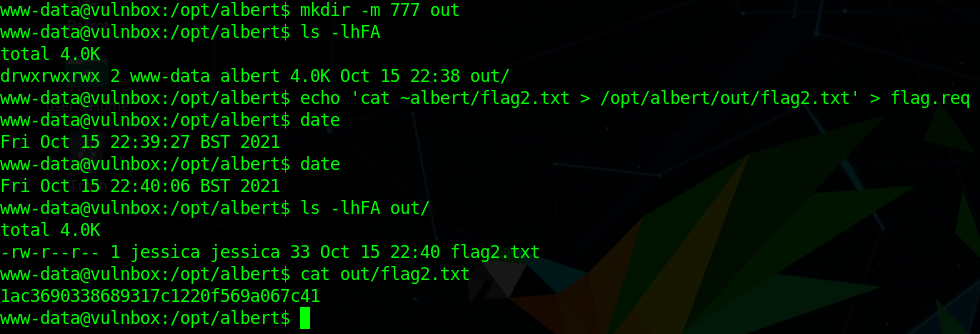
\includegraphics[width=1.00\textwidth]{52-cronjob-cat-flag2.png}
        \caption{\texttt{flag2.txt}}
    \end{figure}

    And we were able to read \texttt{flag2.txt}. Now, let's try to take
    advantage of this situation to get into \textbf{jessica}'s account.

    To achieve this, if possible, we should enumerate what she has or can do. As
    her permissions to her home directory were very restrictive, we may want to
    start to see what's in there:

    \begin{figure}[H]\label{pic:53-cronjob-ls-home}
        \centering
        \includegraphics[width=1.00\textwidth]{53-cronjob-ls-home.png}
        \caption{Listing \textbf{jessica}'s home contents}
    \end{figure}

    There's a \texttt{.ssh} directory, which might have a private key to her own
    account. If we list the contents:

    \begin{figure}[H]\label{pic:54-cronjob-ls-ssh}
        \centering
        \includegraphics[width=1.00\textwidth]{54-cronjob-ls-ssh.png}
        \caption{Listing \textbf{jessica}'s \texttt{.ssh} folder}
    \end{figure}

    There's a \texttt{id\_rsa} file, which is used to store private \textbf{SSH}
    keys. Let's get its contents:

    \begin{figure}[H]\label{pic:55-cronjob-cat-id_rsa}
        \centering
        \includegraphics[width=1.00\textwidth]{55-cronjob-cat-id_rsa.png}
        \caption{Getting \textbf{jessica}'s \texttt{id\_rsa} private key}
    \end{figure}

    Since \textbf{jessica} is the owner of the files we're creating through her
    \textbf{cronjob}, we cannot modify the file, and we need to change the
    permissions to be readable exclusively by the owner to use it. However, we
    can copy the file, as we can read it, and then we're going to be the owner
    of the copy:

    \begin{figure}[H]\label{pic:56-ssh-id_rsa}
        \centering
        \includegraphics[width=1.00\textwidth]{56-ssh-id_rsa.png}
        \caption{Trying to log in with \texttt{id\_rsa}}
    \end{figure}

    At the end of the previous screenshot, I tried to log in with the private
    key, but it asked me for a passphrase\footnote{We were able to tell so
    because in the second line of \texttt{id\_rsa} there was the word
    \texttt{ENCRYPTED}.}, so I cancelled it.

    In this case, we should try to crack it, a well-known option to achieve this
    is by using \verb!ssh2john! which will give us a hash to crack with the
    \texttt{john} utility. As those utilities won't probably be on the victim's,
    we should transfer to our attacking machine and crack it there:

    \begin{figure}[H]\label{pic:57-transfer-id_rsa}
        \centering
        \includegraphics[width=1.00\textwidth]{57-transfer-id_rsa.png}
        \caption{Transferring \texttt{id\_rsa}}
    \end{figure}

    \begin{figure}[H]\label{pic:58-ssh2john}
        \centering
        \includegraphics[width=1.00\textwidth]{58-ssh2john.png}
        \caption{Getting a \texttt{john}-friendly hash from the private key}
    \end{figure}

    And we finally crack it:

    \begin{figure}[H]\label{pic:59-john-id_rsa}
        \centering
        \includegraphics[width=1.00\textwidth]{59-john-id_rsa.png}
        \caption{Cracking the password-protected \texttt{id\_rsa}}
    \end{figure}

    Now, we can log into the machine as \textbf{jessica} through her private
    key:

    \begin{figure}[H]\label{pic:60-ssh-jessica}
        \centering
        \includegraphics[width=1.00\textwidth]{60-ssh-jessica.png}
        \caption{Logging as \textbf{jessica} through \textbf{SSH}}
    \end{figure}

\pagebreak
\subsubsection{Privilege Escalation}

    Note: we're in a restricted bash shell (\texttt{rbash}), which is a little
    uncomfortable, as this machine wasn't secured enough, we can bypass it by
    spawning a bash shell:

    \begin{figure}[H]\label{pic:61-bypassing-rbash}
        \centering
        \includegraphics[width=0.85\textwidth]{61-bypassing-rbash.png}
        \caption{Bypassing a poorly secured \texttt{rbash}}
    \end{figure}

    Enumerating the system as this new user, we find out there's an internal
    service listening on port 25, which is a default port for \textbf{SMTP}, so,
    we check our inbox and we have an unread mail:

    \begin{figure}[H]\label{pic:62-ss}
        \centering
        \includegraphics[width=0.85\textwidth]{62-ss.png}
        \caption{Listing all open ports in the victim machine}
    \end{figure}

    \begin{figure}[H]\label{pic:63-mail-1}
        \centering
        \includegraphics[width=1.00\textwidth]{63-mail-1.png}
        \caption{Reading a mail}
    \end{figure}

    From the mail we know \texttt{sudo} is not installed, but there's a similar
    utility, like \texttt{doas}:

    \begin{figure}[H]\label{pic:64-sudo-vs-doas}
        \centering
        \includegraphics[width=1.00\textwidth]{64-sudo-vs-doas.png}
    \end{figure}

    From the configuration file we see the user \textbf{jessica} can run as
    \textbf{root} the command \texttt{cmp} without providing any password.

    How to abuse this? There's a great resource called
    \href{https://gtfobins.github.io}{GTFOBins} which shows different ways to
    abuse \textit{Linux} binaries depending on certain situations:

    \begin{figure}[H]\label{pic:65-gtfobins-cmp}
        \centering
        \includegraphics[width=1.00\textwidth]{65-gtfobins-cmp.png}
        \caption{Getting info from \textbf{GTFOBins} on how to abuse the binary}
    \end{figure}

    Basically we can compare two files and get the output. With this, we can
    think already what we should do: read the flag.

    I'm not going to do so right now, I have two better purposes. The first one
    is to get shell as \textbf{root}, and the second one is actually explaining
    why I've done what I've done.

    To make the most of it, I think I should start by explaining what I'm going
    to do and why. What I want to do is easy: to read a privileged file, like
    \texttt{/etc/shadow}, where all the password hashes from system users are
    stored, and see if any of them is crackable.

    Take the next image as a simple example on how to read a file with
    \texttt{cmp}:

    \begin{figure}[H]\label{pic:66-cmp-demo}
        \centering
        \includegraphics[width=1.00\textwidth]{66-cmp-demo.png}
        \caption{Simple example on how to read a file with \texttt{cmp}}
    \end{figure}

    About the output format of \verb!cmp -bl!:
    \begin{enumerate}
        \item The first column is the character position to compare.
        \item The second column is the decimal code of the character at the 
            position to compare from the first file.
        \item The third column is the \textbf{ASCII} representation of
            the character at the position to compare from the first file.
        \item The fourth column is the decimal code of the character at the 
            position to compare from the second file.
        \item The fifth column is the \textbf{ASCII} representation of
            the character at the position to compare from the second file.
    \end{enumerate}
    
    I know it seems a mouthful, but basically the order of the arguments matter,
    and we are more interested in the \textbf{ASCII} representation rather than
    their decimal code. And you may have noticed there were some missing
    positions at the far left...

    Notes to take into account:
    \begin{enumerate}
        \item When the same character is found in the same position at both
            files, the output of this is omitted.
        \item \verb!cmp! stops comparing when a
            \textbf{EOF}\footnote{\textbf{EOF}: \textit{End Of File}.} is
            reached.
        \item The \textit{newline} character is represented as \verb!^J!.
    \end{enumerate}

    Knowing this, if we want to leak the whole \texttt{/etc/shadow} contents, we
    need to use a file larger than that one, and make sure any of the characters
    on them match at any position.

    Find a file with this characteristics seems hard, but we can craft one at
    will. We can use the \verb!\0! character which is meant to indicate the end
    of a string and we won't find it in a text file. And we can make it as large
    as we want:

    \begin{figure}[H]\label{pic:67-dd-zero}
        \centering
        \includegraphics[width=0.80\textwidth]{67-dd-zero.png}
        \caption{Crafting a file a special file}
    \end{figure}

    We don't know the size of \texttt{/etc/shadow}, but we know it's not 1
    megabyte.

    To get the \texttt{/etc/shadow} contents:

    \begin{figure}[H]\label{pic:68-cmp-shadow}
        \centering
        \includegraphics[width=1.00\textwidth]{68-cmp-shadow.png}
        \caption{Leaking \texttt{/etc/shadow} with \texttt{cmp}}
    \end{figure}

    \begin{enumerate}
        \item \verb!doas cmp -bl zero.dd /etc/shadow!\newline
            We compare, as \textbf{root}, our crafted file with our target one.
        \item \verb!awk '{print $NF}'!\newline
            We filter the last column, which contains the \textbf{ASCII} value
            of our target file.
        \item \verb!tr -d '\n'!\newline
            We remove the \textit{newline} characters. Otherwise, we would end
            up with one character by line.
        \item \verb!sed 's/\^J/\n/g'!\newline
            We substitute the \verb!^J! character with a \textit{newline}, as
            it's what it actually represents.
        \item \verb!tee shadow!\newline
            We save the output in a file named \texttt{shadow} at the same time
            the output is shown on the screen.
    \end{enumerate}

    Let's try to see if the \textbf{root} password is within
    \texttt{rockyou.txt}. But first, we should transfer the file:

    \begin{figure}[H]\label{pic:69-socat-transfer}
        \centering
        \includegraphics[width=0.80\textwidth]{69-socat-transfer.png}
        \caption{File transfer with \texttt{socat}}
    \end{figure}

    \begin{figure}[H]\label{pic:70-john-shadow}
        \centering
        \includegraphics[width=1.00\textwidth]{70-john-shadow.png}
        \caption{Cracking \textbf{root} password from \texttt{shadow}}
    \end{figure}

    And we have the \textbf{root} password: \textbf{lovelove}.

    Let's get access as \textbf{root} and read the last flag:

    \begin{figure}[H]\label{pic:71-root}
        \centering
        \includegraphics[width=0.85\textwidth]{71-root.png}
        \caption{Gaining \textbf{root} access and reading \texttt{/root/root.txt}}
    \end{figure}


\subsection{Flags}

    albert's flag: 
    \newline
    {\centering\color{Purple}
    \verb!3f440ebbc04e5d97a06383555cd50ba1!
    }
    \newline
    jessica's flag: 
    \newline
    {\centering\color{Purple}
    \verb!1ac3690338689317c1220f569a067c41!
    }
    \newline
    root's flag: 
    \newline
    {\centering\color{Purple}
    \verb!6c52e2288bc30f0fc3cb2a0d8eae6c8d!
    }

\end{document}
